%%Note: You can only use \section command, you are not allowed, per TTU Graduate School, use
%%\subsection command for ghigher level subheadings. At most level 2 subheadings are allowed.
\chapter{Cyber-Physical Systems} 
\label{Cyber-Physical Systems Chapter}

\section[URE Generation Mechanisms]{URE Generation Mechanisms}

Electronic digital circuitry utilizes many periodic signals generated by components such as clocks and oscillators. As part of their inherent operation, these signals are often directly coupled or mixed and modulated both 1) Intentionally for proper operation of the device and 2) Unintentionally resulting from imperfect filtering of high frequency signals or the operation of nonlinear components. This behavior in digital devices leads to generated URE being conducted on to the power infrastructure as shown in Figure \ref{fig:ure_model}. All periodic signals used in the operation of an electronic device are potentially, and independently, filtered by some process before being directly conducted as URE outside the device often through powerline emissions.  Additionally, each periodic signal may mix (multiply) with other periodic signals before being conducted as URE.

\begin{figure}[tb]
	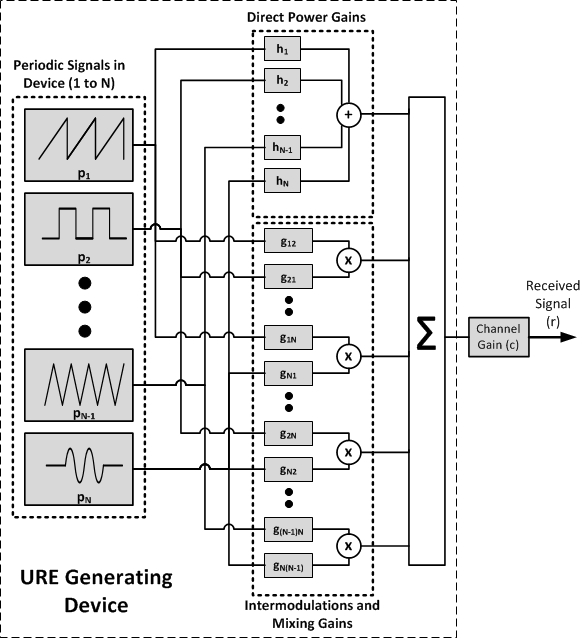
\includegraphics[width=\textwidth]{./model_results/URE_Model.jpg}
	\centering
	\caption{Model of URE generation mechanisms within an electronic device.  URE is composed of the direct conduction components and the intermodulation components of periodic signals utilized within the URE generating device.}
	\label{fig:ure_model}
\end{figure}

The simplified model in Figure \ref{fig:ure_model} does not take in to account the continued mixing and addition of previously multiplied signals which could theoretically continue nearly indefinitely resulting in a significantly increased model complexity.  Given that no assumption was made with regard to the periodic signals ($P_n$), the additional frequency components generated from continued addition and multiplication can be folded in to additional $P$ components or different periodic signal structures. 

\section[Model Development]{Model Development}

Analytically, the received complex URE time domain signal, $r$, can be written as the sum of the direct and intermodulation responses
\begin{equation}
	r ={} c \ast \left(\sum^N_{n=1} p_{n} \ast h_{n} + \sum^N_{i\neq{}j} \left(p_{i} \ast g_{i,j}\right)\left(p_{j} \ast g_{j,i}\right)\right) \label{eq:uremodel1}
\end{equation}
where $r$ is the time domain received signal, $c$ is the URE channel gain, $p_{n}$ are periodic signals used within the devices, $h_{n}$ are the direct power gains for each signal, and $g_{i,j}$ are mixing product gains for component cross-talk and intermodulation, $i$ and $j$ are sequences $1$ to $N$, and $N$ is the number of periodic signals. Note that Equation \ref{eq:uremodel1} assumes no signal mixes with itself.

Using the Convolution Theorem to transform $r$ into its Power Spectral Density (PSD), $\hat{r}$,   
\begin{equation}
    \hat{r} ={} \hat{c} \left( \underbrace{\sum^{N}_{n=1} \hat{p}_{n}\hat{h}_{n}}_\text{Direct Conduction} + \underbrace{\sum^N_{i\neq{}j} \hat{p}_{i}\hat{g}_{i,j} \ast  \hat{p}_{j}\hat{g}_{j,i}}_\text{Mixing Products} \right) \label{eq:uremodel2}
\end{equation}
where $\hat{p}$ is the PSD of $p$ and $\hat{g}$, $\hat{h}$, and $\hat{c}$ are the Fourier transforms of $g$, $h$, and $c$ filter responses, respectively.

Evaluation of the trivial case where $p_1 = \sin(2\pi f_1 t)$, $p_2 = \sin(2\pi f_2 t)$, $c = h_1 = h_2 = g_1 = g_2 = \delta(t)$, and $f_1 \gg f_2$ shows the following 
\begin{equation} \label{eq:uremodelsimpletime}
\begin{split}
	r & = \sin(2\pi f_1 t) + \sin(2\pi f_2 t) + \sin(2\pi f_1 t)\sin(2\pi f_2 t) \\
		& = \sin(2\pi f_1 t) + \sin(2\pi f_2 t) + \frac{1}{2}\cos(2\pi(f_1 - f_2)t) +  \frac{1}{2}\cos(2\pi(f_1 + f_2)t)\\
\end{split}
\end{equation}
which returns the following positive frequency spectral components
\begin{equation} \label{eq:uremodelsimplefreq}
	\hat{r} = \underbrace{\frac{1}{2}\delta(f - f_1) + \frac{1}{2}\delta(f - f_2)}_\text{Unmodulated Frequency Peaks} + \underbrace{\frac{1}{4}\delta\left(f - (f_1 - f_2)\right) + \frac{1}{4}\delta\left(f - (f_1 + f_2)\right)}_\text{Modulation Sidebands}\\
\end{equation}
 
Examination of Equation \ref{eq:uremodelsimplefreq} shows that for the simple case of two periodic signals, two unmodulated frequency tones and two modulation sidebands are present.  The number of potential frequency peaks within a URE spectrum grows at a rate of $\mathcal{O}(n^2)$ for each additional periodic signal and $\mathcal{O}(n^2)$ for each additional harmonic associated with the periodic signals, resulting in combined growth of $\mathcal{O}(n^2) \times \mathcal{O}(n^2) = \mathcal{O}(n^4)$.  For instance, $10$ carriers, with $10$ harmonics each, can generate nearly $10000$ peaks within the frequency domain. The number of potential peaks within the spectrum of a URE signal can be significant, resulting in an overdetermined system with a very large feature space, which DASP is presented to address.   

The continuous-time Fourier Series expansion of a periodic signal shows that it is comprised of an infinite sum of its respective harmonics; therefore, aligning and summing its harmonic content maximizes detection of the signal.  Although the fundamental frequencies of the periodic signals comprising $r$ are unknown, the HASP algorithm provides a method of aligning harmonics of all periodic signals within a given band regardless of the fundamental frequency.  Additionally, the trigonometric product identities show that the intermodulation and mixing of periodic signals results in the sum and differences of the mixing frequencies, as shown in Equation \ref{eq:uremodelsimplefreq}.  The MASP, CMASP, and SCAP algorithms provide a method for detecting these modulations and aligning the frequency mixing sums and differences when the underlying carrier and modulation frequencies are unknown.  As shown in Sections \ref{Harmonically Aligned Signal Projection}, \ref{Modulation Aligned Signal Projection}, \ref{Spectral Correlation Aligned Projection}, \ref{Cross-Modulation Aligned Signal Projection} the HASP, MASP, SCAP, and CMASP algorithms provide a method for aligning and summing harmonics and their cross-products regardless of their underlying fundamental frequency, carrier frequency, and modulation frequency and therefore maximize features relevant to device detection and classification.  Additionally, Section \ref{Frequency Aligned Signal Projection} describes the Frequency Aligned Signal Projection which provides a method for aligning frequencies over time for further characterization of signal harmonic components and their respective time and frequency modulations.

\section[DASP Methodology]{DASP Methodology}

Alignment of signal components, such as harmonics, modulations, and frequencies, with the DASP algorithms result in 2-D images which need to be further processed for extraction of features and eventually used for testing and training in a machine learning framework.   As shown in Figure \ref{fig:dasp_methodology}, raw time domain signal captures are transformed through a DASP process in to a 2-D structure and further processed through an image scaling, segmentation, and summing process.   Statistical features and processed DASP images are then utilized for training and testing using LDA, k-NN, and CNN machine learning processes.  

\begin{figure}[tb]
	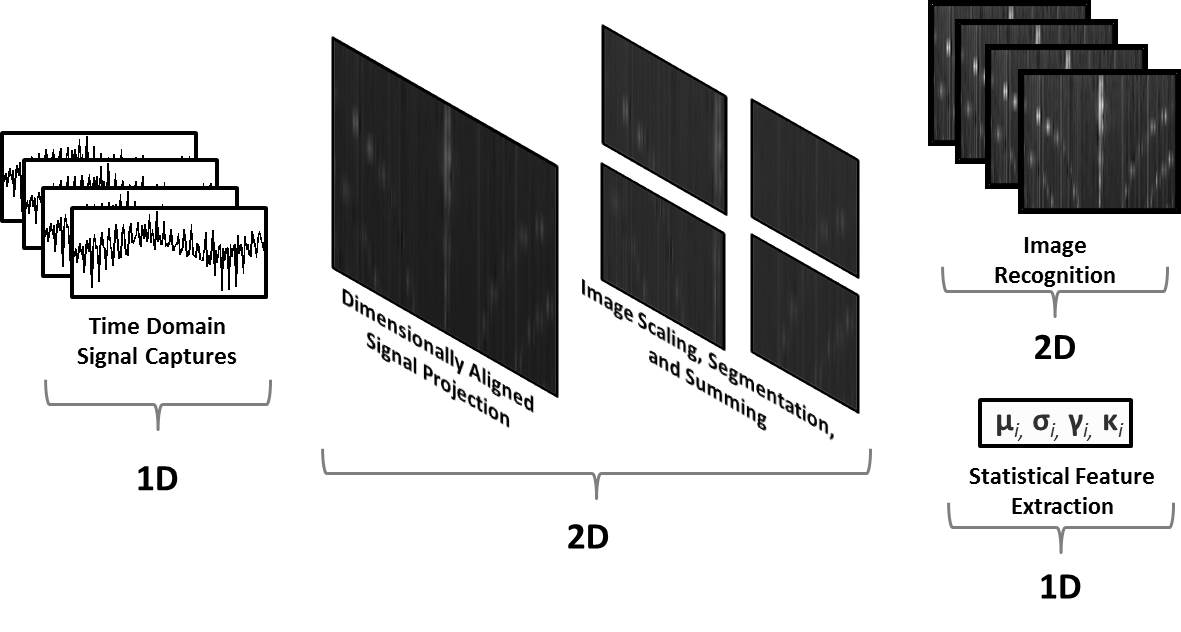
\includegraphics[width=\textwidth]{./model_results/model.jpg}
	\centering
	\caption{DASP processing and feature generation methodology.  The DASP algorithms transform a 1-D vector into a 2-D image which is subsequently transformed, segmented, or processed through an image processing algorithm.  The DASP images are then utilized to classify URE from electrical devices through a variety of feature extraction and learning methods.}
	\label{fig:dasp_methodology}
\end{figure}